%; whizzy chapter
% -initex iniptex -latex platex -format platex -bibtex jbibtex -fmt fmt
% 以上 whizzytex を使用する場合の設定。


%     Tokyo Debian Meeting resources
%     Copyright (C) 2008 Junichi Uekawa
%     Copyright (C) 2008 Nobuhiro Iwamatsu

%     This program is free software; you can redistribute it and/or modify
%     it under the terms of the GNU General Public License as published by
%     the Free Software Foundation; either version 2 of the License, or
%     (at your option) any later version.

%     This program is distributed in the hope that it will be useful,
%     but WITHOUT ANY WARRANTY; without even the implied warranty of
%     MERCHANTABILITY or FITNESS FOR A PARTICULAR PURPOSE.  See the
%     GNU General Public License for more details.

%     You should have received a copy of the GNU General Public License
%     along with this program; if not, write to the Free Software
%     Foundation, Inc., 51 Franklin St, Fifth Floor, Boston, MA  02110-1301 USA

%  preview (shell-command (concat "evince " (replace-regexp-in-string "tex$" "pdf"(buffer-file-name)) "&"))
% 画像ファイルを処理するためにはebbを利用してboundingboxを作成。
%(shell-command "cd image200804; ebb *.png")

%%ここからヘッダ開始。

\documentclass[mingoth,a4paper]{jsarticle}
\usepackage{monthlyreport}

% 日付を定義する、毎月変わります。
\newcommand{\debmtgyear}{2008}
\newcommand{\debmtgmonth}{9}
\newcommand{\debmtgdate}{20}
\newcommand{\debmtgnumber}{44}

\begin{document}

\begin{titlepage}
\thispagestyle{empty}

% タイトルページ:編集必要な部分は最初のマクロに飛ばすこと

\vspace*{-2cm}
第\debmtgnumber{}回 東京エリア Debian 勉強会資料

\hspace*{-2.4cm}
\includegraphics[width=210mm]{image200801/2008title.eps}\\
\hfill{}\debmtgyear{}年\debmtgmonth{}月\debmtgdate{}日

\end{titlepage}

\dancersection{Introduction}{上川 純一}
 
 今月のDebian勉強会へようこそ。これからDebianの世界にあしを踏み入れると
 いう方も、すでにどっぷりとつかっているという方も、月に一回Debianについ
 て語りませんか?

 Debian勉強会の目的は下記です。

\begin{itemize}
 \item \underline{Debian Developer} (開発者)の育成。
 \item 日本語での「\underline{開発に関する情報}」を整理してまとめ、アップデートする。
 \item \underline{場}の提供。
 \begin{itemize}
  \item 普段ばらばらな場所にいる人々が face-to-face で出会える場を提供
	する。
  \item Debian のためになることを語る場を提供する。
  \item Debianについて語る場を提供する。
 \end{itemize}
\end{itemize}		

 Debianの勉強会ということで究極的には参加者全員がDebian Packageをがりがり
 と作るスーパーハッカーになった姿を妄想しています。情報の共有・活用を通し
 て Debianの今後の能動的な展開への土台として、「場」としての空間を提供す
 るのが目的です。

以上を目的とした、2008 年アジェンダです:
\begin{enumerate}
 \item 新年会「気合を入れる」
 \item Open Source Conference Tokyo (3/1)
 \item データだけのパッケージを作成してみる、
       ライセンスの考え方 (David Smith)
 \item バイナリ一つのパッケージを作成してみる (吉田@板橋)\\
       バージョン管理ツールを使いDebianパッケージを管理する(git)\\
       アップストリームの扱い(svn/git/cvs)(岩松 信洋さん)
 \item バイナリの分けたパッケージの作成。(前田さん)\\
       バイナリの分け方の考え方、アップグレードなどの運用とか。
 \item パッケージ作成(dpatch/debhelperで作成するパッケージ)(小林儀匡さん)\\
       OSC 2008 Hokkaido
 \item パッケージ作成(kernel patch、kernel module)(岩松 信洋)
       Debconf発表練習(上川さん)

 \item Debconf アルゼンチン、Debian 温泉、コミックマーケット74

 \item Open Source Conference Tokyo/Fall、
       デーモン系のパッケージの作成、latex、 emacs-lisp、フォントパッケージ
 \item パッケージの cross-compile の方法、amd64 上で i386 のパッケージと
       か、OSC-Fall報告会、Debconf報告会
 \item 国際化 po-debconf / po化 / DDTP
 \item 忘年会
\end{enumerate}


\newpage

\begin{minipage}[b]{0.2\hsize}
 \definecolor{titleback}{gray}{0.9}
 \colorbox{titleback}{\rotatebox{90}{\fontsize{80}{80} {\gt デビアン勉強会} }}
\end{minipage}
\begin{minipage}[b]{0.8\hsize}
\hrule
\vspace{2mm}
\hrule
\tableofcontents
\vspace{2mm}
\hrule
\end{minipage}

\dancersection{事前課題}{岩松 信洋}

今回の事前課題は
\begin{enumerate}
\item Debianで気になった翻訳されていないもの
\item あなたの考えている Debian パッケージメンテナの想像図
\end{enumerate}

というものでした。
その課題に対して下記の内容を提出いただきました。

\subsection{前田さん}
\subsubsection{Debian 気になった翻訳されていないもの}
とりあえずよく使いそうなmanマニュアルでどのくらい翻訳されていないのかをざっと調べてみました。
\begin{itemize}
  \item 無線LAN関係のmanマニュアル
    \begin{itemize}
      \item wireless-toolsパッケージのmanマニュアル。
      \item wpa\_supplicant(8), wpa\_supplicant.conf(5)
      \item wpa\_gui(8)
    \end{itemize}

  \item セキュリティ関連ツールのmanマニュアル。
    \begin{itemize}
      \item gpg(1)
      \item openssl(1ssl) (ところでこれ、何故OPENSSL(1SSL)何でしょうかね?)
      \item tripwire(8), twadmin(8)
      \item ssh(1), sshd(8), sshd\_config(5), ssh\_config(5)
      \item bastille(1m)
      \item chkrootkit(1)
    \end{itemize}
  \item システム管理系のmanマニュアル。
    \begin{itemize}
      \item syslog-ng(8)
      \item inetd(8) (個人的にはinetdはもう使っていないですが、デフォルトでは入ってますよね)
      \item interfaces(5)
      \item logrotate(8)
      \item gshadow(5)
      \item pam(7)
      \item udev(7)
      \item vim(1)
    \end{itemize}
\end{itemize}
面倒になったので途中で調べるの止めました。
有線LANに比べると設定が面倒なので日本語になっていないと一般の人には余計に敷居が上がるだろうと思います。ただ、無線LANとかセキュリティ関連(特にOpenSSHとか)は、Upstreamの更新頻度&一度の変更での差異が大きいのも原因でしょうか。
やることいっぱいありますね…。


\subsection{平澤さん}
\subsubsection{私の考えるDebian パッケージメンテナの想像図}

ほんとに想像でしかかけないのですが..........
お題を3つの単語にわけてみて、想像をふくらましてみます。

まず、``Debian''について。安定性を重視したディストリビューションと聞いている。

きっと、Debianの裏方(メンテナー?)さんが
ライブラリなどの依存関係なんかを細かく確認をしながら
リリースするんだろうなぁ、とか想像する。

次、``パッケージ''. 個別のプログラムをxxx.debファイルにまとめられている状
態を指す?
それとも``current''、``stable'',``testing''と呼ばれている、カテゴリー分けされ
たプログラムの
塊のことを指すのかしら? よくわからない。

次、 ``メンテナ''. 訳するとメンテナンスをする人
想像が想像をよび、すでに妄想の状態かも。

いい仕事をする ``仕事人'' のことを指すのでしょうか?
仕事の一部は定型化されていると想像するので、ルーチンワーク
な部分をやっつけるツールってのがたくさんあるんだろうな?とか想像。

\subsection{やまねさん}
\subsubsection{Debian で気になった翻訳されていないものを教えてください}
gksu, update-manager (すいません、まだやってませんでした…)

\subsection{山本さん}
\subsubsection{Debian で気になった翻訳されていないものを教えてください}
\url{http://www.debian.org} の文書は大体翻訳されてきたと思うけど、
最近は \url{http://wiki.debian.org} で盛んに文書が出されたり、
編集されたりしてるよね。

特に lenny でリリース予定(だっけ?)の armel のページなんかは
\url{http://www.debian.org/ports} から wiki へのリンクぐらいしかない。
当然、翻訳なんかもないが、そろそろなんとかねにゃいかん気もする。
\url{http://wiki.debian.org} で気になるのは、まだまだあるんじゃないかな?


\subsubsection{あなたの考えている Debian パッケージメンテナの想像図}
きっと、スーパーなハカーに違いない!
コーラとピザを片手に、コードを書いているんだ!

\subsection{つじかたさん}
\subsubsection{Debianで気になった翻訳されていないものを教えてください}
CDBSのドキュメント。
以前、CDBSを勉強しようと思ったのですが、日本語ドキュメントが見つからず挫折しました。
今、「入門Debianパッケージ」読んで勉強してます。


\subsection{吉田@板橋さん}

\subsubsection{Debian パッケージメンテナの想像図}
編集者の都合により削除させていただきました。

\subsubsection{Debian で気になった翻訳されていないものを教えてください}
lintianのメッセージ、aptのman,gpgのman。
lintianのメッセージの対処方法(黙らせ方)がぐぐっても、
翻訳サイトに掛けても良くわからない。
日本語にすればわかるのか?といえばそれも微妙だが。
aptitudeのmanは日本語化されているのにaptのmanは日本語化されていない
ぐ(以下略)しても太古のMLの断片が出てくるだけ...
gpg(GnuPG)の日本語man...ぐ(略、現状地球上になさげ。訳してみようと思ったが、
量が多すぎて挫折。

\subsection{たかはし あきゆき さん}
\subsubsection{Debian パッケージメンテナの想像図}
俺はプログラムなんて書けないけど」が口癖の黒魔術士

\subsubsection{Debian で気になった翻訳されていないものを教えてください}
lennyのアップデート・マネージャが気になります。

\subsection{あけどさん}
\subsubsection{Debian で気になった翻訳されていないものを教えてください}
DebianというかUpstreamになるかと思うのですが、rubyやperlのマニュアルページは未だ日本語版が無いようです。
マニュアルページでは他にも日本語版の無い物が色々とありますね。
それと、翻訳とはちょっと違うのですが
\url{http://manpages.debian.net/} で提供されている日本語版のページで文字化けが気になる所です。
Debian関係では、Debian Wiki の日本語化の残っている所がまだまだありますし、
WebドキュメントのDebian Developer's Referenceの日本語ページが
去年から手を着けたまま未完了なのが気になっています。(査読をお手伝い途中のままですみません。)

\subsubsection{あなたの考えている Debian パッケージメンテナの想像図}
具体的な人物が思いつくので想像というよりそのものって感じでしょうか。
なので、詳細については控えさせて頂きたく存じます。


\subsection{hidewon さん}
\subsubsection{あなたの考えている Debian パッケージメンテナの想像図}

いつもパソコンの画面の前に座り、ジャンク
フードを食しながら、あらゆるUNIXコマンドを
あやつり、それらの結果に一喜一憂をし、液晶画面を
みながら明日のソフトウェアを創造しつづけるスーパーハッカー。
とてもすごいひとたち。

パッケージの依存を解決したり、バグが発見されれ
ばそれらを瞬時に解決しなければならないのでしょうか。
英語のパッケージである場合、それらは英語で
作者に問い合わせるなどの折衝役もしなければ
ならないのでしょうか。パッケージが書かれている
言語がじぶんのしらないもので書かれている場合、
それらを自分でなんとかしなければならないのでしょうか。
あるいは修正できるスキルがなければメンテナンスを
してはいけないのでしょうか。プログラミングの経験は
必須なのでしょうか。いったいどんな作業がおこなわれて
いるのか知りたいです。
ときどきソフトウェアの不具合などがあるとき、パッケージを
展開すると知らないひとのなまえとメールアドレスがありました。
あれがメンテナでしょうか。そうだとすればあれがぼくと彼らを
つなぐ唯一の接点でした。
ここへ連絡をとってしまっていいものだろうか?となやむことが
よくあります。メンテナというひとがどんなひとでどんなことを
しているひとなのかということがわからないので、連絡をとるのが
怖かったのです。

メンテナはどんなひとたちでしょうか。


\subsection{森田 尚さん}
\subsubsection{Debianで気になった翻訳されていないもの}
自分が知らないだけかもしれませんが、
\begin{itemize}
  \item jargon - the definitive compendium of hacker slang
  \item fortunes - Data files containing fortune cookies
\end{itemize}
とか。

\subsection{キタハラ さん}
\subsubsection{Debianで気になった翻訳されていないものを教えてください}
{\bf Etch} のGUIインストールをした時に説明文
の中で日本語になってい無い所があったのを思い出した
が、どこだったが思い出せない。 当時のメモを見ると
{\bf uswsusp}の説明が英語で迷った」とあるのでこれ
だと思うが、これを見てもまだ思い出せない。 最近、
いろんな事がありすぎたせいか、歳のせいか?


\subsection{日比野 さん}
\subsubsection{Debianで気になった翻訳されていないものを教えてください}
私の場合のお約束ということで関数型言語系を挙げておきます。
Developing Applications With Objective Camlという
原著がフランス語のOCamlの本の英訳が ocaml-book-en というパッケージにあります。
その英訳がさらに日本語になると嬉しいなあとか。
途中までは \url{http://d.hatena.ne.jp/sumii/20060408/1144492539} に有ったりしますが。

\subsection{岩松}
\subsubsection{Debianで気になった翻訳されていないものを教えてください}
Git, Xfce 全般、awesome
\subsubsection{あなたの考えている Debian パッケージメンテナの想像図}
ツンデレ。

%%% trivia quiz
\dancersection{Debian Trivia Quiz}{岩松 信洋}

ところで、みなさん Debian 関連の話題においついていますか?Debian関連の話
題はメーリングリストをよんでいると追跡できます。ただよんでいるだけではは
りあいがないので、理解度のテストをします。特に一人だけでは意味がわからな
いところもあるかも知れません。みんなで一緒に読んでみましょう。

今回の出題範囲は\url{debian-devel-announce@lists.debian.org} に投稿された
内容とDebian Project Newsからです。
\begin{multicols}{2}
 \subsection{debian-devel-announce}
 \url{debian-devel-announce@lists.debian.org}への投稿内容からです。
 
 \santaku
 {今年も Debconf が開催されました。どこで開催されたでしょうか。}
 {中国}
 {アルゼンチン}
 {スペイン}
 {B}
 % 中国は 北京でオリンピック、スペインは次回、今回はアルゼンチン
 
 \santaku
 {ギブアップ宣言をした Debian サブプロジェクト/チームは何でしょうか}
 {The Debian Live project}
 {The Debian EEEPC team}
 {The Debian Jr. project}
 {C}
 % マンパワーが足りないのと進展がほとんどないため

 \santaku
 {Lenny frozen が宣言されたのはいつでしょうか?}
 {2008/07/26}
 {2008/07/27}
 {2008/07/28}
 {B}
 % HEによってフリーズ宣言
 
 \santaku
 {Andreas Schuldei が立ち上げた新しいチームは何でしょうか。}
 {Debian マーケティング チーム}
 {Debian Dream チーム}
 {Debian Chrome チーム}
 {A}

 \santaku
 {Debian GNU/Linux 4.0 のアップデート版が出ましたが、何と呼ばれているでしょうか。}
 {etch and lenny}
 {etch with you}
 {etch and a half}
 {C}

 \santaku
 {リリースに向けての作業が佳境に入っています。このような作業の中、lennyの次のバージョンとなるリリースのコードネームが決まりました。何でしょうか。}
 {3つ目エイリアン squeeze}% 3つ目エイリアン
 {言葉遊びのオモチャ spell}%言葉遊びのオモチャ
 {重量挙げ選手のアクションフィギュア rocky}%重量挙げ選手のアクションフィギュア
 {A}

\end{multicols}
\dancersection{最近のDebian関連のミーティング報告}{岩松 信洋}
\subsection{東京エリアDebian勉強会43回目報告}
8月の第43回東京エリアDebian勉強会を実施しました。 
勉強会として、今回の Debconf 開催地である アルゼンチンからIRCを使って行われました。
今回の参加者は Debconf からは 上川さん、日本からは 武藤さん、やまねさん、山本さん、
小室さん、本庄さん、藤沢さん、前田さん、あけどさん、岩松が参加しました。
上川さんをHubにして、Debian 関係に関しての質問などが行われました。
詳細は、第43回Debian勉強会資料としてまとめましたので、そちらを参照してください。

\subsection{Debian 温泉報告}
2008年8月16日はDebian 15 周年でした。おめでとう! Debian 勉強会では、15周年を祝うために
有志で Debian 温泉と題した 合宿を行いました。
今回は、Debian勉強会に参加された方から希望者を募って実験的に合宿を行う方式を取りました。
参加者はやまねさん、あけどさん、前田さん、小林儀匡さん、山本 浩之さん、日比野 啓さん、鈴木さん、岩松の8人でした
当初は伊豆の伊東温泉で行う予定でしたが、予定していた場所を予約できず、
急遽、草津温泉に変更なりました。伊東温泉を楽しみにしていた方、申し訳ございませんでした。
詳細は、第43回Debian勉強会資料としてまとめましたので、そちらを参照してください。

\subsection{コミックマーケット74}
今年の夏もコミックマーケット74 で Debian勉強会資料を販売しました。
今回からページ数が大幅に増え、120ページ。今まで行ってきた製本方法では冊子にできないため、くるみ製本にして
販売しました。販売数は50冊で完売することができました。
委託販売していただいた USAGI補完計画さん、編集に協力していただいた方、
どうもありがとうございました。ちなみに166円の赤字でした。

\subsection{第90回 カーネル読書会:Debianパッケージ入門の入門}
急遽 YLUG が主催する カーネル読書会 で やまねさんが {\bf Debianパッケージ入門の入門}
ということで発表しました。Debian関係の方からDebian勉強会に参加された
事のある方、パッケージに興味があって参加された方など多方面から参加者として集まり、やまねさん
につっこみを入れていました。いろいろ課題の残る発表でしたが、無事終えることができました。
この発表で興味を持ってくれた方が増えて、Debian/Ubuntu界隈が盛り上がればいいなと思っています。
やまねさんの次回発表(反省会)に期待したいと思います。

% (query-replace-regexp "<.*?>" "")
% (query-replace-regexp "^[	 ]\+" "")


\dancersection{Po4a でドキュメント翻訳の保守を楽にしよう}{小林 儀匡}
\label{sec:po4a}
\index{po4a}

翻訳の保守は新規翻訳よりも手間のかかる作業になりがちです。
しかし、これを怠ると原文との乖離は大きくなり、折角の翻訳も価値が下がっていきます。
Debianで開発されているPo4aは、プレーンテキスト、XML、HTML、LaTeX、nroff (man)
など様々な形式のドキュメント翻訳をPOという形式で管理し、保守性を上げるツールです。
今回はこのPo4aの使い方と、
新たなドキュメント形式をPOで管理するために知っておくべき内部構造について説明します。

\subsection{はじめに 〜地味で地道なドキュメント翻訳保守作業〜}

長期的に見れば、ドキュメント翻訳者の作業で最も大変で最も大切なのは、
ドキュメントの翻訳作業ではなく翻訳の{\bf 保守}作業でしょう。
何週間、何ヶ月もの作業の末、1万行を超える長いドキュメントの翻訳作業を終えたとしても、
原文が変わり続ける限り、保守をしなければ翻訳の価値は下がっていきます。

保守は地味で地道な作業です。
原文に対しては、次のような変更が発生します。

\begin{itemize}
 \item 訳文には影響のないtypoの修正
 \item 記述の追加・変更・削除 (修正を含む)
 \item パラグラフの位置の変更
 \item マークアップの変更 (マークアップ言語で書かれたドキュメントの場合)
\end{itemize}

同時に、次のような非本質的な変更も頻繁に発生します。

\begin{itemize}
 \item パラグラフのインデントの変更
 \item パラグラフの改行位置の変更 (主に語句の挿入・変更・削除に起因する)
\end{itemize}

こういった様々な種類の変更は大抵は混ざっています。
ドキュメントの翻訳者は通常、\texttt{diff}で差分を眺めて変更を把握し、
それを翻訳に反映させます。
差分を読んで変更を把握する能力によって、翻訳に反映させる作業が楽にも大変にもなります。

% FIXME: まだ書く

このようなドキュメント翻訳の保守作業に必要な労力を和らげてくれるのがPo4aです。
Po4aは、様々な形式のドキュメント翻訳をPOという形式で一括して管理し、
保守性を上げるツールです。
以下では、まずPOというファイル形式が、翻訳にとってどのように便利なのかを説明し、
その上でPo4aがどのようなツールなのか説明します。

\subsection{PO}

POは、プログラムのメッセージの翻訳のために作られたファイル形式です。
ここではその書式や編集用のツールについて見ていきましょう。

\subsubsection{POの基本的な書式}

まずは、POの基本的な書式を説明します。

POには、原文と訳文の対からなるエントリが空行区切りで多数収められています。
最初に、簡単なエントリの例を紹介します。

\begin{commandline}
#: src/apt_config_treeitems.cc:99
msgid ""
"%BOption:%b  %s\n"
"%BDefault:%b %s\n"
"%BValue:%b   %s\n"
msgstr ""
"%Bオプション:%b %s\n"
"%Bデフォルト:%b %s\n"
"%B値:%b         %s\n"
\end{commandline}

一目瞭然ですが、\texttt{msgid}から始まる一連の行、\texttt{msgstr}から始まる一連の行の、
\texttt{"}で囲まれた部分は、それぞれ原文と訳文です。
%"

「\texttt{\#}」で始まる行は基本的にすべてコメントです。
特に「\texttt{\#:}」で始まる行は、原文を抽出した位置を示す参照用の行です。
これは\texttt{xgettext}がメッセージを抽出してPOTを生成するときに設定します。
翻訳者は、\texttt{msgid}を見ても理解できない場合、
この参照コメントをもとにしてソースコードを眺めることができます。

「\texttt{\#:}」以外にも、様々な種類のコメントがあります。
そのようなコメントを含んだエントリの例を紹介します。

\begin{commandline}
# 最後の %s は「 (core dumped)」。
#. ForTranslators: "%s update %s" gets replaced by a command line, do not translate it!
#: src/generic/apt/download_update_manager.cc:383
#, c-format
msgid "The debtags update process (%s update %s) was killed by signal %d%s."
msgstr ""
"debtags 更新プロセス (%s update %s) がシグナル %d に kill されました%s。"
\end{commandline}

「\texttt{\#.}」で始まる行は、
原文のメッセージと一緒にソースコードから抽出されたコメントです。
主に、メッセージの翻訳に注意が必要な場合やメッセージが翻訳しにくい場合に、
開発者から翻訳者への説明に使われます。
これも\texttt{xgettext}がメッセージ抽出時に設定します。

「\texttt{\#,}」で始まる行はフラグです。
最もよく使われるフラグはfuzzyというフラグでしょう。
これについては後述します。
これは様々なツールが設定します。

それ以外の、
「\texttt{\#}」の後に何の記号もない行は、翻訳者が翻訳作業時に勝手に追加したコメントです。
各エントリにはこのような翻訳者コメントを自由自在につけることができます。

このようなコメント情報は、
プログラムのソースコードに書くコメントと同様、人間の作業にのみ必要となるものなので、
MOに変換するときにすべて削除されます\footnote{したがって、\texttt{msgunfmt}でMOをPOに変換すると、コメントをまったく含まないPOが得られます。}。

\subsubsection{fuzzyエントリ}

\texttt{msgmerge}が古いPOに新しいPOTをマージする際、
既に翻訳されているエントリの\texttt{msgid}に似た\texttt{msgid}を持つエントリが追加されることがあります。
例えば、エントリAの\texttt{msgid}に似た\texttt{msgid}を持つエントリA'が追加されるとします。
このとき、\texttt{msgmerge}はAをベースとしてA'を翻訳できると判断し、
A'の\texttt{msgstr}にAの\texttt{msgstr}の内容を設定した上で、
A'にfuzzyフラグをつけます。
このようにして作られるエントリが、次のような{\bf fuzzyエントリ}です。

\begin{commandline}
#: src/main.cc:181
#, fuzzy, c-format
msgid ""
" -q             In command-line mode, suppress the incremental progress\n"
"                indicators.\n"
msgstr " -q                コマンドラインモードで進行状況を逐一表示しません。"
\end{commandline}

しかしこれだけだと、翻訳者には、\texttt{msgid}がどう変化したのか分かりません。
そこでGNU gettextのバージョン0.16から導入されたのが、
次のような、「\texttt{\#|}」で始まるコメントです。

\begin{commandline}
#: src/main.cc:181
#, fuzzy, c-format
#| msgid ""
#| " -q             In command-line mode, suppress the incremental progress "
#| "indicators."
msgid ""
" -q             In command-line mode, suppress the incremental progress\n"
"                indicators.\n"
msgstr " -q                コマンドラインモードで進行状況を逐一表示しません。"
\end{commandline}

「\texttt{\#|}」で始まるコメントは、以前の\texttt{msgid}です。
\texttt{msgmerge}に\texttt{--previous}を指定した場合に設定されます。
このコメントを使えば、
以前の\texttt{msgid}と現在の\texttt{msgid}を比較できるので、
どのような変更を\texttt{msgstr}に加えれば翻訳を現在の\texttt{msgid}に対応できるのかが簡単に分かります。
POの保守性を上げる仕組みと言えます。
\texttt{msgmerge}に\texttt{--previous}が指定されていない場合は指定しておくとよいでしょう。

\subsubsection{ヘッダ}

翻訳を扱う際、
翻訳者やその連絡先、原文の問題の連絡先、翻訳の更新日時、文字セットなどは重要なメタ情報です。
POでは、最初のエントリを{\bf ヘッダ}として使用し、
そのエントリの\texttt{msgstr}にこれらのメタ情報を含めることになっています。
ヘッダの\texttt{msgid}は空文字列にすると決まっています。

また、著作権情報など、書式が曖昧な情報や長い情報は、
ヘッダのコメント (つまりファイルの冒頭) に書くことになっています。

以下は、aptitudeのja.poの例です。

\begin{commandline}
# Japanese translations for aptitude
# aptitude の日本語訳
# Copyright (C) 2006-2008 Noritada Kobayashi <nori1@dolphin.c.u-tokyo.ac.jp>.
# This file is distributed under the same license as the aptitude package.
#
msgid ""
msgstr ""
"Project-Id-Version: aptitude 0.4.1\n"
"Report-Msgid-Bugs-To: aptitude@packages.debian.org\n"
"POT-Creation-Date: 2008-09-05 16:05+0200\n"
"PO-Revision-Date: 2008-05-16 03:35+0900\n"
"Last-Translator: Noritada Kobayashi <nori1@dolphin.c.u-tokyo.ac.jp>\n"
"Language-Team: Japanese\n"
"MIME-Version: 1.0\n"
"Content-Type: text/plain; charset=UTF-8\n"
"Content-Transfer-Encoding: 8bit\n"
"Plural-Forms: nplurals=1; plural=0;\n"
\end{commandline}

なお、ここでは省略しましたが、筆者は、
メッセージカタログ内での用語統一を容易にするため、
aptitudeやSubversionなど大規模なPOでは、ヘッダのコメントに対訳表を含めています。

\subsubsection{その他の書式}

ここまでで、POのエントリの書式についてざっと見ました。

POのエントリについては、\texttt{msgid}と\texttt{msgstr}から成るもの以外にも、
複数形への対応として\texttt{msgid}、\texttt{msgid\_plural}、\texttt{msgstr[n]}から成るものがあります。
詳しくはGNU gettextのドキュメント\footnote{\texttt{gettext-doc}パッケージ。}の『3 The Format of PO Files』を参照してください。

\subsubsection{PO編集ツール}

POで翻訳作業を行うにはPO編集ツールが便利です。
POはテキストなのでどんなテキストエディタでも編集できますが、
翻訳に含まれる「\texttt{"}」や「\verb@\@」を手でエスケープするのは厄介です。%"
そのような機械的な処理は、POに特化したPO編集ツールに任せるのがよいでしょう。
また、PO編集ツールには翻訳支援機能を持つものもあるので、
作業効率も上がるはずです。

PO編集ツールとしてよく知られているのは、
EmacsのPO専用メジャーモードであるpo-mode、
KDEのPO編集スイートであるKBabel、
GNOMEのPOエディタであるGtranslator、
そしてpoeditです。

ここでは、筆者が慣れているpo-modeについて、筆者がよく使う操作だけざっと説明します。
説明中で何度も登場する「選択エントリ」とは「現在カーソルがあるエントリ」の意味です。

まず、エントリ間の移動には以下のようなキー操作が使えます。

\begin{description}
 \item[\texttt{n}] 次のエントリに移動します。
 \item[\texttt{p}] 前のエントリに移動します。
 \item[\texttt{t}] 次の既訳エントリに移動します。
 \item[\texttt{T}] 前の既訳エントリに移動します。
 \item[\texttt{f}] 次のfuzzyエントリに移動します。
 \item[\texttt{F}] 前のfuzzyエントリに移動します。
 \item[\texttt{u}] 次の未訳エントリに移動します。
 \item[\texttt{U}] 前の未訳エントリに移動します。
 \item[\texttt{o}] 次のobsoleteエントリに移動します。
 \item[\texttt{O}] 前のobsoleteエントリに移動します。
 \item[\texttt{m}] 選択エントリの位置をスタックにpushします。
 \item[\texttt{r}] スタックからpopして得られたエントリに移動します。
\end{description}

また選択エントリの操作には以下のようなキー操作が使えます。

\begin{description}
 \item[\texttt{RET}] 編集用バッファを開いて、選択エントリの\texttt{msgstr}を編集します。
 \item[\texttt{\#}] 編集用バッファを開いて、選択エントリの翻訳者コメントを編集します。
 \item[\texttt{k}] 選択エントリの\texttt{msgstr}をカット (kill) します。
 \item[\texttt{K}] 選択エントリの翻訳者コメントをカット (kill) します。
 \item[\texttt{w}] 選択エントリの\texttt{msgstr}をコピーします。
 \item[\texttt{W}] 選択エントリの翻訳者コメントをコピーします。
 \item[\texttt{y}] 選択エントリの\texttt{msgstr}にペースト (yank) します。
 \item[\texttt{Y}] 選択エントリの翻訳者コメントにペースト (yank) します。
 \item[\texttt{TAB}] 選択エントリのfuzzyフラグを取り除きます。
 \item[\texttt{DEL}] 選択エントリが既訳の場合はfuzzyフラグをつけます。
	    未訳またはfuzzyの場合はobsoleteにします。
	    obsoleteの場合は削除します。
 \item[\texttt{C-j}] 選択エントリの\texttt{msgid}の内容を\texttt{msgstr}にコピーします。
 \item[\texttt{s}] 選択エントリの参照コメントをもとにソースコードの該当行を表示します。
	    参照コメントに複数の位置が記述されている場合は、順番に表示します。
\end{description}

編集用バッファでは通常のEmacsの編集操作ができます。
特殊な操作は以下のとおりです。

\begin{description}
 \item[\texttt{C-c C-c}] 編集用バッファの内容を\texttt{msgstr}または翻訳者コメントの内容として設定し、バッファを閉じます\footnote{もちろん、この変更はメインバッファで保存操作を行うまで保存されません。}。
 \item[\texttt{C-c C-k}] 編集用バッファの内容を破棄してバッファを閉じます。
\end{description}

最後に、メインバッファでのPO全体に関わる操作は以下のとおりです。

\begin{description}
 \item[\texttt{\_}] 行った変更を取り消します。
 \item[\texttt{?}, \texttt{h}] ヘルプを表示します。
 \item[\texttt{V}] \texttt{msgfmt}に\texttt{--check} (\texttt{-c}) をつけて実行し、POに問題点がないか確認した上で保存します。
	    例えば、\texttt{msgid}が改行記号で終わっているのに\texttt{msgstr}が改行記号で終わっていない場合、それが報告されます。
\end{description}

\begin{figure}[htbp]
 \begin{center}
  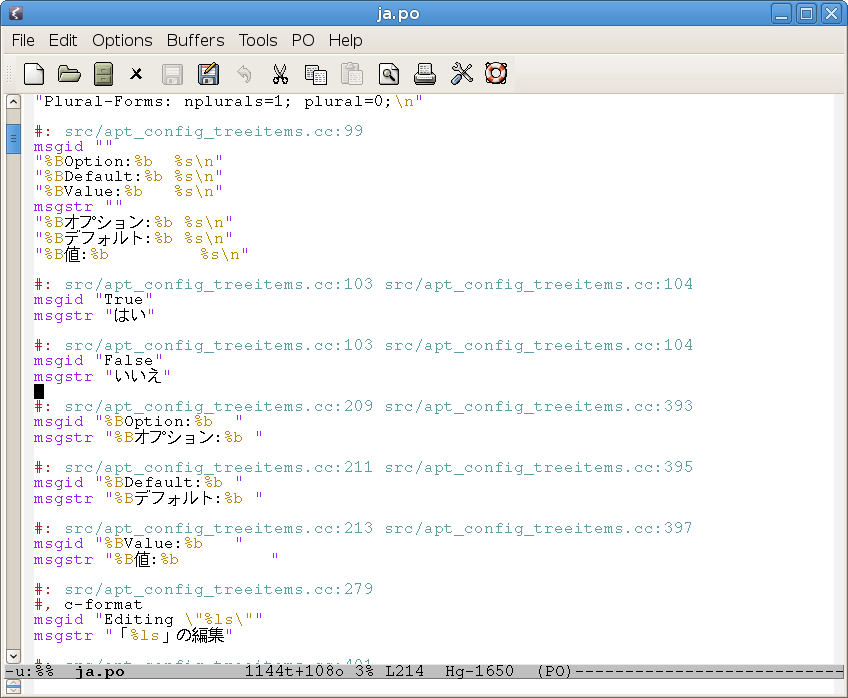
\includegraphics[width=0.4\hsize]{image200809/po-mode.png}
  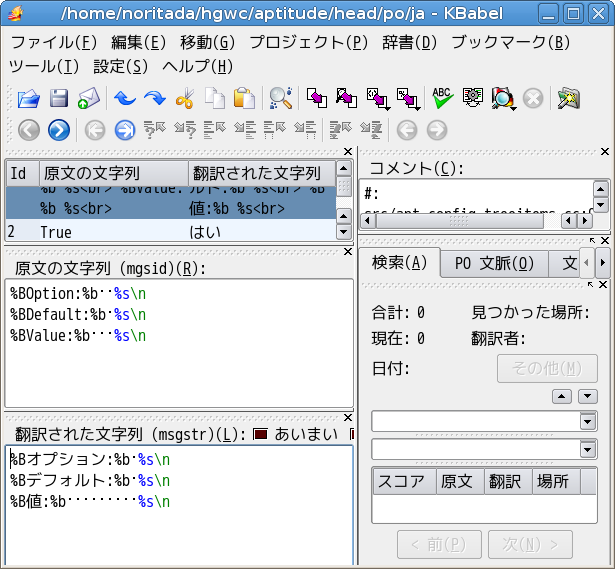
\includegraphics[width=0.4\hsize]{image200809/KBabel.png}
 \end{center}
 \caption{po-modeとKBabel}
 \label{fig:po-editors}
\end{figure}

以上の簡単な説明から分かると思いますが、po-modeは移動や編集がしやすく、
非常に便利です。

ただ、po-modeには今のところ翻訳メモリのような機能はありません。
KBabelやGtranslatorは翻訳メモリを備えているので、
翻訳メモリに興味のあるかたはこれらを試してみるのもよいでしょう。

\subsubsection{GNU gettextツール群}

翻訳作業にはPO編集ツールを使うことになるでしょうが、
一方でGNU gettextが提供する、
POやPOTに対してコマンドラインから自動処理できるツール群も、知っておくと便利です。
以下でざっと説明します。

\begin{description}
 \item[\texttt{msgattrib}] エントリの状態に応じた一括処理をします。
	    例えば、「fuzzyエントリのみにする」、「fuzzyエントリからfuzzyフラグを取り除く」といったことが可能です。
 \item[\texttt{msgcat}] 複数のPOを繋げます。
 \item[\texttt{msgcmp}] POとPOTが含む\texttt{msgid}セットを比較します。
 \item[\texttt{msgcomm}] 複数のPOに含まれる共通の\texttt{msgid}を抽出します。
 \item[\texttt{msgconv}] POの文字セットを変換します。
 \item[\texttt{msgen}] 英語のPOを作成します。
	    入力ファイルの未訳のエントリの\texttt{msgstr}に、\texttt{msgid}と同じ文字列を設定します。
 \item[\texttt{msgexec}] POに含まれるすべての翻訳に対してコマンドを実行します。
 \item[\texttt{msgfilter}] POに含まれるすべての翻訳に対して共通の処理をします。
 \item[\texttt{msgfmt}] POをコンパイルしてMOに変換します。
 \item[\texttt{msggrep}] パターンにマッチしたエントリをPOから抽出します。
 \item[\texttt{msginit}] POを初期化します。
 \item[\texttt{msgmerge}] POにPOTをマージします。
 \item[\texttt{msgunfmt}] MOからPOに逆コンパイルします。
 \item[\texttt{msguniq}] POに含まれる重複した\texttt{msgid}を1つにまとめます。
 \item[\texttt{xgettext}] ソースコードから\texttt{msgid}を抽出してPOTを生成します。
\end{description}

開発者が主に使うのは\texttt{xgettext}と\texttt{msgmerge}、\texttt{msgfmt}ですが、
他のツールも使いこなせるようになっておくと便利です。
使い方は各ツールのマニュアルページを参照してください。

\subsubsection{まとめ}

POはプログラム翻訳のために作られたファイル形式で、参照コメントのような翻訳に有用な情報や、
fuzzyエントリのような翻訳作業・保守作業の効率を上げるための仕組みを含んでいることを説明しました。
また、POという書式に特化した編集ツールについても説明しました。

\subsection{ドキュメント翻訳でPOを使うという考え方}

プログラム翻訳のために生み出されたPOは、
翻訳者にとって翻訳と保守の両方の作業をしやすい環境を提供する存在となりました。
その理由としては以下のようなものが考えられます。

\begin{itemize}
 \item PO自体に翻訳と保守を支援するための仕組みがある上、
       翻訳支援機能を持つPO編集ツールも存在する。
 \item メッセージの管理はツールがやってくれるので、人間は翻訳の管理に集中していればよい。
       \begin{itemize}
	\item メッセージがソースコードのどこにあるかが翻訳者にとって重要でないので、
	      メッセージがソースコード内で移動しても翻訳者は気にする必要がない。
	\item \texttt{msgmerge}でPOを更新すると、どのエントリの翻訳を更新すべきか瞬時に分かり、
	      PO編集ツールでそのエントリへ簡単に移動できる。
       \end{itemize}
\end{itemize}

一方でドキュメント翻訳については、通常は原文をそのままコピーして翻訳作業を開始するため、
翻訳以外の部分 (インデント、ドキュメント内での位置など) に変更があった場合、
その影響を翻訳者が受けます。
プログラム翻訳と比べて分量が多いのに保守性が低いので、
結果として翻訳者への負担は非常に大きくなります。
この状況は、翻訳者にとって大きな悩みの種でした。

そこで生まれたのが、ドキュメント翻訳に対してもPOを使おうという考え方です。
具体的には、ドキュメントの各ブロックをエントリとしたPOを作り、
ドキュメントとPOとを相互変換できるようにすることで、
翻訳者がPOでの翻訳管理に集中できるようにします。
以下のツールがそのような思想で作られています。

\begin{description}
 \item[Po4a] Debianで開発されている\footnote{厳密に書くと、Debian Projectのメンバーが、
	    同プロジェクトが提供しているフリーソフトウェアプロジェクトホスティングサービスであるAlioth上で、
	    1つのプロジェクトとして開発しています。}。
	    対象とするドキュメント形式は、プレーンテキスト、XML、HTML、LaTeX、nroff (man)、Podなど多数で、
	    Perlで書かれたモジュールおよびプログラムの集合として実装されている。
	    Debianパッケージは\texttt{po4a}。
 \item[poxml] KDEで、KDE SDKモジュールの1つのコンポーネントとして開発されている。
	    対象とするドキュメント形式はDocBook XMLで、C++で実装された、
	    \texttt{po2xml}、\texttt{xml2pot}などの実行可能プログラムから成る。
	    Debianパッケージは\texttt{poxml}。
 \item[xml2po] GNOMEでgnome-doc-utilsの1つのユーティリティとして開発されている。
	    対象とするドキュメント形式はDocBook XMLである。
	    Pythonで実装されたシンプルな1つのファイルから成るので、
	    手軽にドキュメントのビルドに使用できる。
	    Debianでは\texttt{gnome-doc-utils}パッケージに含まれる。
\end{description}

poxmlやxml2poがDocBook XMLのみを扱うツールであるのに対し、
Po4aが様々な形式をサポートしているのは、
おそらくGNOMEやKDEとDebianの立場の違いを反映しているのでしょう。
GNOMEやKDEはプロジェクト内でドキュメント形式をDocBook XMLに統一できますが、
ディストリビュータであるDebianでは、
様々なソフトウェアの様々なドキュメントに対応する必要があるのです。

以降のセクションでは、ドキュメント翻訳にPOを使用する3つのツールのうち、
唯一複数のドキュメント形式をサポートしているPo4aについて見ていきます。

\subsection{Po4aの基本}

Po4aというソフトウェア名は、「po for anything」から来ています。
名前からも分かるように、
最初から様々なドキュメント形式の翻訳をPOで管理することを目的としており、
そのために入力形式として複数の形式を扱うことを想定した作りとなっています。

例えば、以下のような形式が現在サポートされています。

\begin{description}
 \item[KernelHelp] カーネル設定ヘルプのドキュメント形式です。
 \item[nroff] Unixの伝統あるマニュアルページの形式です。
	    BSDマニュアルページで使用されているmdoc形式もサポートされています。
	    初心者が読み書きしにくい形式ですが、
	    Po4aでサポートされたので、
	    インラインのマークアップだけ分かれば (原文の真似をすれば) 翻訳できます。
 \item[POD] Perl関連のドキュメントに使われる形式です。
	    ソースコードの横にコメントとして書き込まれたドキュメントは翻訳しにくいですが、
	    それをPOとして抽出し、翻訳しやすくします。
 \item[SGML] 最近ではXMLのほうが主流ですが、一昔前のドキュメント形式の主流です。
	    現在サポートされているDTDはDebianDoc-SGMLとDocBook SGMLのものです。
 \item[TeX/LaTeX] 著名な組版ソフトウェア\LaTeX{}の形式です。
 \item[GNU Texinfo] GNUのドキュメントに使用される形式です。
 \item[XML] 最近よく使われるドキュメント形式です。
	    現在サポートされているDTDはDia、DocBook XML、Guide XML、XHTMLのものです。
\end{description}

サポートされている形式の一覧は、
\texttt{po4a-gettextize}、\texttt{po4a-translate}、\texttt{po4a-updatepo}などのコマンドに\texttt{--help-format}オプションを与えると表示できます\footnote{残念ながら今のところ\texttt{po4a}コマンドに与えることはできないようです。}。
コマンドに\texttt{--format} (\texttt{-f}) などを与えてドキュメント形式を指定する場合、
この一覧に載っている名前を使用してください。

\begin{commandline}
noritada[3:39]%  po4a-gettextize --help-format   terra:~/svnwc/build-common/doc
有効フォーマット一覧:
  - dia: 非圧縮 Dia ダイアグラム。
  - docbook: Docbook XML。
  - guide: Gentoo Linux の xml ドキュメントフォーマット。
  - ini: .INI フォーマット。
  - kernelhelp: 各カーネルのコンパイルオプションのヘルプメッセージ。
  - latex: LaTeX フォーマット。
  - man: 古き良きマニュアルページフォーマット。
  - pod: Perl オンラインドキュメントフォーマット。
  - sgml: debiandoc と docbook DTD の双方。
  - texinfo: info ページフォーマット。
  - tex: 汎用 TeX ドキュメント (latex を参照)。
  - text: シンプルなテキストフォーマット。
  - wml: WML ドキュメント。
  - xhtml: XHTML ドキュメント。
  - xml: 汎用 XML ドキュメント (docbook を参照)。
\end{commandline}

\subsection{Po4aの使い方}

\subsubsection{導入(1): 原文ドキュメントファイルからPOTを生成する}

Po4aを使ってドキュメントの翻訳をする場合、最初にすべきことは、
原文のドキュメントファイルからPOTを生成することです。
POTの生成には\texttt{po4a-gettextize}コマンドを使用します。
\texttt{-f}オプションの引数にドキュメントファイルの形式を、
\texttt{-m}オプションの引数に原文ドキュメントファイル ({\bf マスタードキュメント}) の名前を、
\texttt{-p}オプションの引数に出力するPOTのファイル名を与えて、コマンドを実行します。
\texttt{-M}オプションの引数で、原文ドキュメントファイルの文字セットを指定することも可能です。

特に問題がない場合はすんなりとコマンドの実行が終了し、POTが生成されます。
ドキュメントの構造に問題がある場合 (例えばXMLにおいてタグがきちんと閉じられていない場合) はエラーになります。

POTが生成されたら、翻訳作業はプログラム翻訳の場合と同じです。
POTをコピーしてPOを作成し、ヘッダを適切に設定した上で翻訳作業を始めましょう。

\paragraph{例}
次の例では、\texttt{hoge.en.html}というXHTMLドキュメントから\texttt{hoge.pot}を生成しています。

\texttt{hoge.en.html} (入力):

\begin{commandline}
<?xml version="1.0" encoding="utf-8" ?>
<!DOCTYPE html PUBLIC "-//W3C//DTD XHTML 1.0 Strict//EN"
"http://www.w3.org/TR/xhtml1/DTD/xhtml1-strict.dtd">
<html xmlns="http://www.w3.org/1999/xhtml" lang="en" xml:lang="en">
<head>
<title>Test file</title>
</head>
<body>
<h1>Test file</h1>
<p>This is an <a href="apple">apple</a>.</p>
<p>This is an <a href="orange">orange</a>.</p>
</body>
</html>
\end{commandline}

コマンドライン:

\begin{commandline}
noritada[14:14]%  po4a-gettextize -v -f xhtml -m hoge.en.html -p hoge.pot    
\end{commandline}

\texttt{hoge.pot} (出力):

\begin{commandline}
# SOME DESCRIPTIVE TITLE
# Copyright (C) YEAR Free Software Foundation, Inc.
# This file is distributed under the same license as the PACKAGE package.
# FIRST AUTHOR <EMAIL@ADDRESS>, YEAR.
#
#, fuzzy
msgid ""
msgstr ""
"Project-Id-Version: PACKAGE VERSION\n"
"POT-Creation-Date: 2008-09-20 14:21+0900\n"
"PO-Revision-Date: YEAR-MO-DA HO:MI+ZONE\n"
"Last-Translator: FULL NAME <EMAIL@ADDRESS>\n"
"Language-Team: LANGUAGE <LL@li.org>\n"
"MIME-Version: 1.0\n"
"Content-Type: text/plain; charset=utf-8\n"
"Content-Transfer-Encoding: ENCODING"

# type: Attribute 'xml:lang' of: <html>
#: hoge.en.html:4 hoge.en.html:4
msgid "en"
msgstr ""

# type: Content of: <html><body><h1>
#: hoge.en.html:6 hoge.en.html:9
msgid "Test file"
msgstr ""

# type: Content of: <html><body><p>
#: hoge.en.html:10
msgid "This is an <a href=\"apple\">apple</a>."
msgstr ""

# type: Content of: <html><body><p>
#: hoge.en.html:11
msgid "This is an <a href=\"orange\">orange</a>."
msgstr ""
\end{commandline}

\subsubsection{導入(2): 原文・翻訳ドキュメントファイルからPOを生成する}

原文と同じ形式で翻訳したドキュメントが既にあり、
それをPo4a用のPOに移行したい場合にも、\texttt{po4a-gettextize}が使えます。
「POTをコピーしてPOを作った上で、
翻訳ドキュメントの各ブロックをコピー・アンド・ペーストでPOの各エントリに埋め込む」という、
間違いなくうんざりする作業は不要です。

ただしこの場合、どの原文がどの訳文に対応するかをPo4aが把握する必要があるので、
{\bf 原文ドキュメントファイルと翻訳ドキュメントファイルが同じ構造である}ことが前提になります。
「同じ構造」とは、Po4aが切り分ける単位、つまりブロックのレベルで見たときに、
対応する要素が同じ順序で並んでいる、という意味です。
もし翻訳側でブロックの追加や削除が行われていたら、変換はエラーで終わるでしょう。
一部のブロックの順序が入れ替わっている場合、変換は見た目は無事に終わるかもしれませんが、
入れ替わったブロックの\texttt{msgid}と\texttt{msgstr}の対応関係はおかしくなっているはずです。

訳注や翻訳者情報を別個のブロックとして翻訳ドキュメントに追加している場合、
それは一旦取り除いてください。
Po4aでは、POから翻訳ドキュメントを生成する際に、
原文にはない要素を追加する方法が提供されています。
方法については後述します。

原文ドキュメントファイルと翻訳ドキュメントファイルが同じ構造であれば、
\texttt{po4a-gettextize}を用いた変換は成功するはずです。
\texttt{-f}オプションの引数にドキュメントファイルの形式を、
POTを生成する場合の一連のオプションに加えて、
\texttt{-l}オプションの引数に翻訳ドキュメントファイルの名前を与えてコマンドを実行します。
\texttt{-L}オプションの引数で、翻訳ドキュメントファイルの文字セットを指定することも可能です。

変換に成功すると、すべてのエントリにfuzzyフラグが設定されたPOが生成されます。
すべてのエントリにfuzzyフラグが設定されるのは、
「ざっとでもいいので、ユーザには変換後にすべてのエントリの原文と訳文を確認してほしい」という開発者の意図を反映したものです
ユーザが自由に編集できる普通のドキュメントに少し制限を与えてPo4aの管理下に置く\footnote{例えば、「ブロックの順序など全体的な構造を原文に合わせる必要がある」、「原文の同じ内容のブロックには、同じ訳文を当てる必要がある」など。}際には、
何かしらの問題が発生している可能性があるのです。

\paragraph{例}
以下では、先程の\texttt{hoge.en.html}に対応する日本語訳\texttt{hoge.ja.html}をPOに変換することを試みます。

まずは、とりあえず\texttt{po4a-gettextize}を実行してみました。

\texttt{hoge.ja.html} (入力):

\begin{commandline}
<?xml version="1.0" encoding="utf-8" ?>
<!DOCTYPE html PUBLIC "-//W3C//DTD XHTML 1.0 Strict//EN"
"http://www.w3.org/TR/xhtml1/DTD/xhtml1-strict.dtd">
<html xmlns="http://www.w3.org/1999/xhtml" lang="ja" xml:lang="ja">
<head>
<title>テストファイル</title>
</head>
<body>
<h1>テスト用のファイル</h1>
<p>これは<a href="apple">リンゴ</a>です。</p>
<p>これは<a href="orange">オレンジ</a>です。</p>
<p>(訳注: オレンジはミカンとは違います。)</p>
</body>
</html>
\end{commandline}

コマンドライン:

\begin{commandline}
noritada[14:54]%  po4a-gettextize -v -f xhtml -m hoge.en.html -l hoge.ja.html -p ja.po
po4a gettextize: Original has less strings than the translation (6<7). Please 
               fix it by removing the extra entry from the translated file. You 
               may need an addendum (cf po4a(7)) to reput the chunk in place 
               after gettextization. A possible cause is that a text duplicated 
               in the original is not translated the same way each time. Remove 
               one of the translations, and you're fine.
po4a gettextization: Structure disparity between original and translated files:
msgid (at hoge.en.html:6 hoge.en.html:9) is of type 'Content of: 
<html><body><h1>' while
msgstr (at hoge.ja.html:6) is of type 'Content of: <html><head><title>'.
Original text: Test file
Translated text: テストファイル
(result so far dumped to gettextization.failed.po)
The gettextization failed (once again). Don't give up, gettextizing is a subtle 
art, but this is only needed once to convert a project to the gorgeous luxus 
offered by po4a to translators.
Please refer to the po4a(7) documentation, the section "HOWTO convert a 
pre-existing translation to po4a?" contains several hints to help you in your 
task
\end{commandline}

訳注を独立したパラグラフにしたためにPOへの変換が失敗したと考え、
訳注の行を削ってもう一度\texttt{po4a-gettextize}を実行してみます。
入力ファイルの内容は省略します。

コマンドライン:

\begin{commandline}
noritada[14:55]%  po4a-gettextize -v -f xhtml -m hoge.en.html -l hoge.ja.html -p ja.po
po4a gettextization: Structure disparity between original and translated files:
msgid (at hoge.en.html:6 hoge.en.html:9) is of type 'Content of: 
<html><body><h1>' while
msgstr (at hoge.ja.html:6) is of type 'Content of: <html><head><title>'.
Original text: Test file
Translated text: テストファイル
(result so far dumped to gettextization.failed.po)
The gettextization failed (once again). Don't give up, gettextizing is a subtle 
art, but this is only needed once to convert a project to the gorgeous luxus 
offered by po4a to translators.
Please refer to the po4a(7) documentation, the section "HOWTO convert a 
pre-existing translation to po4a?" contains several hints to help you in your 
task
\end{commandline}

なんだか変なエラーが出てしまっています。
どうも、\texttt{title}と\texttt{h1}の原文がともに「Test file」なのに、
一方の訳は「テストファイル」で、他方の訳が「テスト用のファイル」となっていることに原因があるようです。
そこで、両方の訳を統一して\texttt{po4a-gettextize}にかけると、変換に成功します。

\texttt{hoge.ja.html} (入力):

\begin{commandline}
<?xml version="1.0" encoding="utf-8" ?>
<!DOCTYPE html PUBLIC "-//W3C//DTD XHTML 1.0 Strict//EN"
"http://www.w3.org/TR/xhtml1/DTD/xhtml1-strict.dtd">
<html xmlns="http://www.w3.org/1999/xhtml" lang="ja" xml:lang="ja">
<head>
<title>テストファイル</title>
</head>
<body>
<h1>テストファイル</h1>
<p>これは<a href="apple">リンゴ</a>です。</p>
<p>これは<a href="orange">オレンジ</a>です。</p>
</body>
</html>
\end{commandline}

コマンドライン:

\begin{commandline}
noritada[15:07]%  po4a-gettextize -v -f xhtml -m hoge.en.html -l hoge.ja.html -p ja.po
\end{commandline}

\texttt{ja.po} (出力):

\begin{commandline}
# SOME DESCRIPTIVE TITLE
# Copyright (C) YEAR Free Software Foundation, Inc.
# This file is distributed under the same license as the PACKAGE package.
# FIRST AUTHOR <EMAIL@ADDRESS>, YEAR.
#
#, fuzzy
msgid ""
msgstr ""
"Project-Id-Version: PACKAGE VERSION\n"
"POT-Creation-Date: 2008-09-20 15:07+0900\n"
"PO-Revision-Date: YEAR-MO-DA HO:MI+ZONE\n"
"Last-Translator: FULL NAME <EMAIL@ADDRESS>\n"
"Language-Team: LANGUAGE <LL@li.org>\n"
"MIME-Version: 1.0\n"
"Content-Type: text/plain; charset=utf-8\n"
"Content-Transfer-Encoding: ENCODING"

# type: Attribute 'xml:lang' of: <html>
#: hoge.en.html:4 hoge.en.html:4
#, fuzzy
msgid "en"
msgstr "ja"

# type: Content of: <html><body><h1>
#: hoge.en.html:6 hoge.en.html:9
#, fuzzy
msgid "Test file"
msgstr "テストファイル"

# type: Content of: <html><body><p>
#: hoge.en.html:10
#, fuzzy
msgid "This is an <a href=\"apple\">apple</a>."
msgstr "これは<a href=\"apple\">リンゴ</a>です。"

# type: Content of: <html><body><p>
#: hoge.en.html:11
#, fuzzy
msgid "This is an <a href=\"orange\">orange</a>."
msgstr "これは<a href=\"orange\">オレンジ</a>です。"
\end{commandline}

\subsubsection{POと原文ドキュメントファイルから翻訳ドキュメントファイルを生成する}

\texttt{po4a-translate}

\subsubsection{原文ドキュメントファイルの更新をPOに反映させる}

\texttt{po4a-updatepo}

\subsubsection{POと翻訳ドキュメントファイルを一括更新する}

\texttt{po4a}

\subsubsection{原文にない要素を翻訳ドキュメントファイルに挿入する}

\subsection{Po4aの内部構造}

\subsubsection{TransTractor::parse()}

\dancersection{【でびあん】Debian パッケージメンテナというお仕事【現在募集中】}{やまね ひでき}

\label{sec:dm-yamane}
\index{dm-yamane}

\subsection{Debian パッケージメンテナのお仕事}

 実は、Debian パッケージのメンテナになるにはそんなに敷居は高くありません。よっぽど入学試験/就職/転職活動の方が難しいと思うほどです。恐れることはありません。多少なりとも興味がある方はこれからの説明をご覧ください。

\subsection{メンテナになる前の下準備}

\begin{enumerate}
 \item GPG 鍵を作っておく (aptitude install gpg \&\& gpg --gen-key)
 \item 公的な身分証明書を用意しておく
 \item 先ほど作った GPG 鍵と身分証明書を利用して、既存の Debian Developer とGPG キーサインの交換を行っておく
 \item メンテナや Developer として問題ないと見なされる作業をしておく (contribute!)
\end{enumerate}

この4つだけ準備したら、さぁ、メンテナになる作業の始まりです。


\subsection{The way to Debian package maintainer}

メンテナになる方法としては2点あります。

\begin{enumerate}
 \item 自分から「このソフトを Debian パッケージにしたい」と申請する
 \item 既存のパッケージのメンテナからメンテナンスを引き継ぐ
\end{enumerate}

 1. は ITP (Intent To Package) という形で行います。特に RFP (Request For Package) という形でユーザから「このソフトを Debian パッケージにして欲しいなぁ」という声に答えるのが望ましいでしょう。

 2. は RFH (Request For Help、協力者募集中)、RFA (Request for Adoption、新メンテナ募集中) や O (Orphaned、みなしご化) というステータスになったパッケージに対して「自分がメンテナになります」と宣言します。

 ITP, RFP, RFA, Orphaned は全て Debian Bug Tracking System (BTS) で管理登録されます (BTS の使い方についてはそのうち別途)。これらを総称して「作業が望まれるパッケージ (Work-Needing and Prospective Packages; WNPP)」と呼びます。この WNPP、BTS で追うのは結構辛いので wnpp.debian.net \footnote{ \url{http://wnpp.debian.net} ではパッケージ化希望されているものや、メンテナが引き取り手を募集しているパッケージを検索できます。
\begin{itemize}
 \item ページの見た目は良くない ;-)
 \item RSSで状況が取得できるので、RSS reader で適宜ピックアップにてチェックすることをお勧めします。
\end{itemize}} を使いましょう。各略語の意味などについては \url{http://www.jp.debian.org/devel/wnpp/} をご覧ください。


\subsubsection{ITP、RFP パッケージ化}

 大抵1からパッケージ化作業ですので、ウェブサイトからソースを取得してライセンスを確認の上、パッケージ作りのお作法に従ってパッケージを作成します。パッケージを作成する際は、unstable 環境の lintian で warning などが出なくなるよう (Debian Policy Manual に準拠するよう) に頑張りましょう。パッケージが作成できたら pbuilder でクリーンルーム環境でビルド可能かどうか (Build-Depends に間違いが無いか) のチェックを行います。問題なくビルドできたら piuparts を使ってインストール/アンインストールで問題が無いか (Depends や preinst,postinst,prerm,postrm スクリプトに問題が無いか) を確認しましょう。ここまで来て問題なければ「Eat your own dog food」、つまり自分の環境にパッケージを入れて問題が起きないかどうかチェックするとベストでしょう。

\begin{screen}
\paragraph*{ライセンスについて}
 ちなみに一番大変なのはここでの「ライセンス確認」作業だと個人的には思っています。そのソフトのウェブページににちょっと書いてあることを鵜呑みにしたりすると、実は中身は全然違うライセンスだ、とか、実はリンクするライブラリとは矛盾するライセンスだ、とかがありますし、英訳ライセンスがないと Debian のパッケージ管理者 (ftpmaster) がライセンス的にそのパッケージを受け入れるかどうかの判断がそもそも出来ませんので必ず適当な英訳ライセンスへの翻訳作業が必要です。

 ライセンスは、独自ライセンスよりも一般的に FLOSS の代表的ライセンス (GPL, BSD, MIT, Artistic など) を使う方が全ての利害関係者にとって利益があるでしょう。何故ならば、ライセンスは「プロトコル」のようなものであり、既存プロトコルを利用する方が新たにプロトコルを実装するよりもはるかに容易に取り扱えるからです。代表的ライセンスでは目的が達成できないときにのみ、独自ライセンスを利用するのが賢いやり方です。
\end{screen}

\subsubsection{RFA, Orphan への対処}

 すでに現在のメンテナが引き継ぎ手を募集している状態 (RFA) や、完全にギブアップor興味を失ってしまった (Orphan) になったパッケージについては、BTS を利用してパッケージを引き取る旨の宣言 (ITA, Intend To Adapt) を行いましょう。加えて関連のメーリングリストで「自分がやろうと思うけど、どう?」と聞いてみるとさらに良いでしょう。合意がとれたら、debian/changelog にて該当の RFA/Orphan バグを閉じるエントリを追記しておきます。大抵の場合は色々とバグレポートが溜まっているので片付けて同様に changelog に記載しておきましょう。


\subsection{アップロード}

 ここまでが終わったらアップロードを行います。Debian Developer であればパッケージを dput や dupload と呼ばれるコマンドを使って、作成されたソースパッケージとバイナリパッケージを直接 Debian へアップロードします。そうでない場合は適当な場所にアップロードして、Debian Developer に代理アップロードをお願いしましょう (アップロード先は、\url{http:://mentors.debian.net}、代理アップロード依頼先は \url{debian-devel@debian.or.jp} がおすすめです)。 

\begin{commandline}
dupload -t anonymous-ftp-master ccspatch_1.6.4-20080903-1_i386.changes
\end{commandline}

 この時点でツールは dsc ファイルや changes ファイルに gpg 署名されているかどうかをチェックして、されていない場合はアップロードしないなどしてくれます。

 サーバ側では、まず「既にあるパッケージの更新なのか、それとも新規パッケージなのか」の判断を行います。新規パッケージの場合は NEW Queue (\url{http://ftp-master.debian.org/new.html}) と呼ばれる所に自動的に移されて、ftpmaster が逐次入れてよいものかどうかのチェックを行っています。おおよそこの工程は1、2週間程度かかります。

 チェックは特にライセンスの問題が無いかについてなどが争点となります。この作業は高度な判断が要求されるため、人的リソース的にボトルネックになりやすいところと、拒否された場合に「何故このパッケージが拒否されたのか」の記録が容易にトラッキングできないのが問題点です。人的リソースについては、アクティブなメンバーを入れることで以前と比較しても改善がされており、トラッキングについては最近になってシステマチックにチェック可能なように提案が出てきているところです。

 更新パッケージについては、サーバ側でソースパッケージの gpg 署名をチェックなどをして「本当にこれは入れていいものかどうか」を判断してダメな場合は reject されます。このチェックについては、アップロード後にサーバから受け入れ/拒否のメールが届きます。

まずアップロードされたパッケージの処理を始めたよ、というメール

\begin{commandline}
From: Archive Administrator <dak@ftp-master.debian.org>
Subject: Processing of ccspatch_1.6.4-20080903-1_i386.changes

ccspatch_1.6.4-20080903-1_i386.changes uploaded successfully to localhost
along with the files:
  ccspatch_1.6.4-20080903-1.dsc
  ccspatch_1.6.4-20080903.orig.tar.gz
  ccspatch_1.6.4-20080903-1.diff.gz
  linux-patch-tomoyo_1.6.4-20080903-1_all.deb

Greetings,

	Your Debian queue daemon
\end{commandline}


チェックして incoming repository に入れたよ、というメール

\begin{commandline}
From: Debian Installer <installer@ftp-master.debian.org>
Subject: ccspatch_1.6.4-20080903-1_i386.changes ACCEPTED

Accepted:
ccspatch_1.6.4-20080903-1.diff.gz
  to pool/main/c/ccspatch/ccspatch_1.6.4-20080903-1.diff.gz
ccspatch_1.6.4-20080903-1.dsc
  to pool/main/c/ccspatch/ccspatch_1.6.4-20080903-1.dsc
ccspatch_1.6.4-20080903.orig.tar.gz
  to pool/main/c/ccspatch/ccspatch_1.6.4-20080903.orig.tar.gz
linux-patch-tomoyo_1.6.4-20080903-1_all.deb
  to pool/main/c/ccspatch/linux-patch-tomoyo_1.6.4-20080903-1_all.deb


Override entries for your package:
ccspatch_1.6.4-20080903-1.dsc - source devel
linux-patch-tomoyo_1.6.4-20080903-1_all.deb - extra admin

Announcing to debian-devel-changes@lists.debian.org


Thank you for your contribution to Debian.
\end{commandline}

 これでパッケージのアップロードが完了しました。BTS に記載されているバグを修正した旨を debian/changelog に適切なスタイルで記述しておくと、BTS から bug closed のメールがやってきます。


\subsubsection{その他アップロードに関する注意}

 ちなみに、Debian バージョンのみの更新の場合 (foo 1.0-1 から foo 1.0-2 への更新など) はオリジナルのソースファイル (orig.tar.gz) をアップロードしないことになっています。もし、orig.tar.gz をアップロードした場合は後から拒否のメールが届きます。

 あと注意として、ライブラリファイルや他の多くのパッケージと関連しているようなパッケージで更新をかけると unstable 環境が壊れるような場合は、experimental へアップロードして関係者と調整することが推奨されています。


\subsection{メンテナンス作業}

 BTS を通じてユーザからバグ報告メールが来るので、それに対応してパッケージの debian ディレクトリ以下を更新して、修正出来たら changelog に完了した旨を記載しておきます (dch コマンドが便利です)。特に RC (Release Critical) バグは早めに修正しましょう。バグが他のパッケージと関連する場合は適当なメーリングリストで関係者と対応を協議して進めていきます。場合によっては、自分のパッケージのバグではなく、他のパッケージのバグである場合もありますので、その場合はバグを BTS で reassign しておきます。パッケージとしてのバグではなく、元々のソース由来のバグの場合は、バグを upstream (開発元) に転送するかパッチを作って upstream と協議しましょう。

 そして upstream での更新に合わせてパッケージも更新します。upstream の更新は debian/watch ファイルを適切に記載していれば、DEHS (Debian External Health Status、\url{http://dehs.alioth.debian.org}) によって定期的にチェックされ、Debian Quality Assuarance の developer ページ (\url{http://qa.debian.org/developer.php}) で状況を確認できます (あとは upstream のリリースアナウンスが流れるメーリングリストに入っておくと良いでしょう)。きちんと設定された debian/watch ファイルがあれば、パッケージによっては更新がものの1分も経たずに出来ます。

 チーム制でメンテナンスをするような場合は共有 repository に更新したソースを忘れずに commit しておきましょう。commit 出来ない場合は、チームのメーリングリストにパッチを送ります。幾度か適切なパッチを送りつづけていると、いつの間にか commit 権が与えられていることが多い様です。

 なお、バグ修正や Debian Policy に適合するために Debian パッケージ側で色々とパッチを当てている (dpatch や quilt を利用する) と新バージョン側のソースとコンフリクトを起こしてその修正に時間がかかることがありますので、なるべく upstream の開発者とメーリングリストなどを通じて普段からコンタクトを取り合っておいて、パッチ自体が取り込まれて不要になるように働きかけましょう。

 この様にしてパッケージ化、メンテナンス等をメンテナは日々行っていきます。特に問題なく時間が経過したパッケージは unstable から testing に移行され、次のリリースを待つことになります。そして、リリースの日を迎えたパッケージは stable へと移されます。


\subsection{特殊な場合}

 以下に頻繁には起きないはずの、ちょっと変わった場合の対応を挙げておきます。

\subsubsection{NMU}

 Non-Maintainer Upload の略で、既存のメンテナ以外の人間がバグ修正のためにパッケージをアップロードすることを指します。あまり頻繁に NMU があるようなパッケージについては、メンテナが本当に活動しているのかどうかをチェックした方がいいでしょう。

\subsubsection{FREEEEEEZE!!}

 特にリリース前には「システム全体の安定化」が必要なため、freeze、つまりパッケージの unstable から testing への自動移行が停止されます。しかし、freeze の間に発覚した、そのままリリースされてしまっては困るようなバグの修正が必要な場合もあります。その場合は リリースマネージャ (RM) に対して「私のこのパッケージを testing に入れるようにしてください!」とお願いします。これを「unblock (exception) request」と一般に呼びます。やり方としてはメーリングリストで RM が理解しやすいフォーマットでメールを投げるだけです。

\begin{commandline}
To: debian-release@lists.debian.org
subject: Please unblock <package> <version>

\begin{itemize}
 \item changelog の抜粋
 \item 理由
 \item debian-devel-announce で流れている freeze exception のどれに当てはまるのか
 \item このアップデートによって何が改善されるのか
 \item このアップデートでは regression が起きない説明
 \item その他、RM が納得してくれるような内容
\end{itemize}

\end{commandline}

 うまくすれば RM から "unblocked" という素っ気ないメールが届きます。これが来たら大成功です。今 unstable にあるパッケージは testing へ移行することが可能になります。


\subsection{メンテナ権の移譲}

 パッケージメンテナも人の子、残念ながら諸事情によりメンテナンスが出来なくなるような事態が起きるかもしれません。なるべく一人でメンテナンスせずチームあるいは自分以外の詳しい/信用できるメンテナもアップロードできるようにしておきます。具体的には debian/control の Uploaders フィールドにアップロードしてもいい人の名前とメールアドレスを書いておきます (GPG 署名に使うものと同一である必要があります)。

\begin{commandline}
Source: ttf-vlgothic
Section: x11
Priority: optional
Maintainer: Debian Fonts Task Force <pkg-fonts-devel@lists.alioth.debian.org>
Uploaders: Hideki Yamane (Debian-JP) <henrich@debian.or.jp>
DM-Upload-Allowed: yes
Build-Depends: debhelper (>= 5)
Build-Depends-Indep: defoma, bzip2
Standards-Version: 3.8.0
Homepage: http://dicey.org/vlgothic/
Vcs-Svn: svn://svn.debian.org/pkg-fonts/packages/ttf-vlgothic/
Vcs-Browser: http://svn.debian.org/wsvn/pkg-fonts/packages/ttf-vlgothic/
\end{commandline}

 そして、メンテナンスが出来なくなりそうな場合は、あまり粘らずにさっさと宣言 (RFA, Orphan) しておきましょう。宣言が無いと「このパッケージ古いな」という悪評が立つだけ…という結果になりかねません。なお、日本の首相と違ってメンテナは頻繁に交代してもきちんとした理由があれば文句は言われることはありません :-) (できれば最初の方から複数人でのチームメンテナンスなどしておくと困ったことになる確率は減ります)


\subsection{終わりに}
 如何でしたか?パッケージメンテナというお仕事がどのようなものか、多少理解が深まっていただければ幸いです。


\clearpage





%\printindex

\cleartooddpage

\vspace*{15cm}
\hrule
\vspace{2mm}

\includegraphics[width=2cm]{image200502/openlogo-nd.eps}
\noindent \Large \bf Debian 勉強会資料\\ \\
\noindent \normalfont \debmtgyear{}年\debmtgmonth{}月\debmtgdate{}日 \hspace{5mm}  初版第1刷発行\\
\noindent \normalfont 東京エリア Debian 勉強会 (編集・印刷・発行)\\
\hrule


\end{document}
